%!TEX encoding = UTF-8 Unicode
%%%%%%%%&%%%%%%%%%%%%%%%%%%%%%%%%%%%%%%%%%%%%%%%%%%%%%%%%%%%%%%%%%%%%%%%%%%%%%%%%%%
%%% 卒業論文
%%% name
%%%%%%%%&%%%%%%%%%%%%%%%%%%%%%%%%%%%%%%%%%%%%%%%%%%%%%%%%%%%%%%%%%%%%%%%%%%%%%%%%%%
\documentclass[a4paper,12pt,oneside,openany,uplatex,dvipdfmx]{jsarticle}

%settings for tables
\setcounter{topnumber}{4}
\setcounter{bottomnumber}{4}
\setcounter{totalnumber}{4}
\setcounter{dbltopnumber}{3}

\renewcommand{\topfraction}{.95}
\renewcommand{\bottomfraction}{.90}
\renewcommand{\textfraction}{.05}
\renewcommand{\floatpagefraction}{.95}

%packages
\usepackage{amsmath, amssymb} %複雑な数式などを打つときに使用
\usepackage{bm, bbm, here} %数式環境内で太字を使うときに便利
%\usepackage{graphicx} %画像を挿入したり,テキストや図の拡大縮小・回転を行う
\usepackage{subfigure} %図を並べる
\usepackage{verbatim} %入力どおりの出力を行う
\usepackage{ascmac} %テキストを枠で囲んだりできるが,微小なズレがでたりする
\usepackage{makeidx} %索引を作成できる
\usepackage{dcolumn} %表の数値を小数点で桁を揃える
\usepackage{lscape} %図表を90度横に倒して配置する
\usepackage{setspace} %行間調整
\usepackage{mathrsfs}
\usepackage[dvipdfmx]{graphicx,hyperref}
\usepackage{pxjahyper}
\usepackage{fancyhdr}
\usepackage{url}
\pagestyle{myheadings}
\makeatletter
\@addtoreset{equation}{section}
\def\theequation{\thesection.\arabic{equation}}
\renewcommand{\thefigure}{
\thesection.\arabic{figure}}
\@addtoreset{figure}{section}
\renewcommand{\thetable}{
\thesection.\arabic{table}}
\@addtoreset{table}{section}
\makeatother

%setting for margins
\setlength{\textwidth}{160truemm}      % テキスト幅: 210-(25+25)=160mm
\setlength{\fullwidth}{\textwidth}     % ページ全体の幅
\setlength{\oddsidemargin}{25truemm}   % 左余白
\addtolength{\oddsidemargin}{-1truein} % 左位置デフォルトから-1inch
\setlength{\topmargin}{15truemm}       % 上余白
\setlength{\textheight}{242truemm}     % テキスト高さ: 297-(25+30)=242mm
\addtolength{\topmargin}{-1.0truein}     % 上位置デフォルトから-1inch

\renewcommand{\labelenumi}{(\arabic{enumi}) } %enumerate環境を1. 2.の形式から(1) (2)の形式へ変更(文書全体).
\setcounter{tocdepth}{2} %項レベルまで目次に反映させるコマンド.

\begin{document}
%!TEX encoding = UTF-8 Unicode
%%%%%%%%&%%%%%%%%%%%%%%%%%%%%%%%%%%%%%%%%%%%%%%%%%%%%%%%%%%%%%%%%%%%%%%%%%%%%%%%%%%
%%% 卒業論文
%%% name
%%%%%%%%&%%%%%%%%%%%%%%%%%%%%%%%%%%%%%%%%%%%%%%%%%%%%%%%%%%%%%%%%%%%%%%%%%%%%%%%%%%
\begin{titlepage}
\begin{spacing}{2.3}
{\large 令和4年度}\\
\hspace{4mm}{\large 卒業研究}\\
\begin{center}
\vspace{100truept}
{\LARGE TITLE}\\ % タイトル
{\LARGE TITLE}\\
\vspace{150truept}
{\LARGE 大阪大学\ 工学部\ 応用理工学科}\\ %所属
{\LARGE マテリアル生産科学科目\ マテリアル科学コース}\\ %所属
{\LARGE 計算材料設計学領域\ number\ name}\\ % 学籍番号
\end{center}

\end{spacing}
\end{titlepage}
 
\pagenumbering{roman}
%%% \begin{abstruct} %ここに概要を記入
%%% \end{abstruct}
\tableofcontents %この位置に目次を作成
\newpage
\clearpage

\pagenumbering{arabic}

\section{緒言}\label{sec:introduction}
\markboth{\ref{sec:introduction} 緒言}{\ref{sec:introduction} 緒言}


\newpage
\section{理論}\label{sec:theory}
\markboth{\ref{sec:theory} 理論}{\ref{sec:theory} 理論}

文章中で数式を使いたい時には\$\$で囲む。$A=B+C$

% equation
\begin{align}
	{\hat{\mathcal{H}}}^{\mathrm{QP}} = \cfrac{1}{2} \sum_{ij} \lvert \psi_i^{\mathrm{QP}} \rangle \left( \mathrm{Re} \Sigma_{ij} (\varepsilon_{i}^{\mathrm{QP}}) + \mathrm{Re} \Sigma_{ij}(\varepsilon_j^{\mathrm{QP}}) \right) \langle \psi_j^{\mathrm{QP}} \rvert
\end{align}

\newpage
\section{結果}\label{sec:results}
\markboth{\ref{sec:results} 結果}{\ref{sec:results} 結果}

\subsection{サブセクション}\label{subsec:label}
\markboth{\ref{subsec:label}サブセクション}{\ref{subsec:label}サブセクション}
% figure
\begin{figure}[H] 
   \centering
   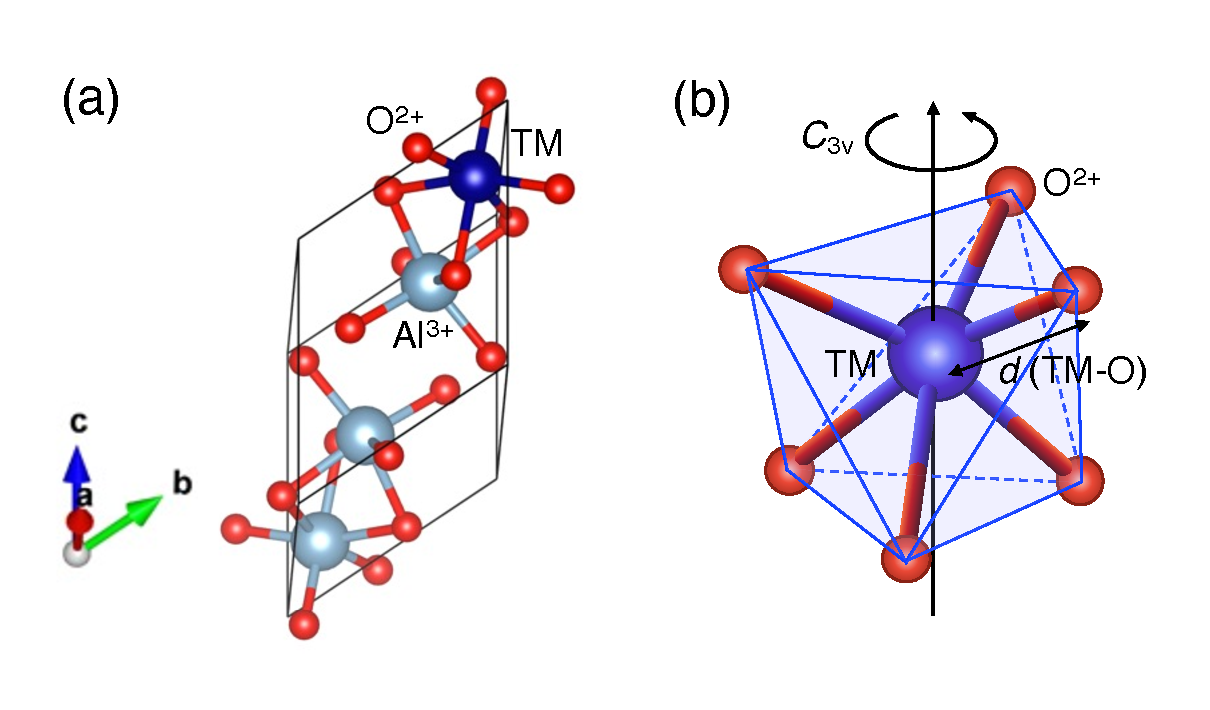
\includegraphics[clip, width=10cm]{img/ruby_local_struc.pdf} 
   \caption{\textbf{$\mathrm{\alpha}$-$\mathrm{Al_2O_3}$の局所構造:} }
   \label{fig:ruby_loca_struc}
\end{figure}

% list up
\begin{enumerate}
	\item 物質依存のパラメータやモデルを必要としない計算手法であること
	\item 半導体・絶縁体のバンドギャップを正確に再現すること
	\item 母物質のバンドと$3d$不純物バンドの位置関係を正確に再現すること
\end{enumerate}

\subsubsection{サブサブセクション}\label{subsubsec:label}

% table
\begin{table}[H]
  \centering
    \caption{\textbf{希土類窒化物における最近接交換相互作用・Curie温度の計算結果}}
    \begin{tabular}{cccc}  \hline 
    REN & $J/k_\mathrm{B}[K]$ &  $T_\mathrm{C}[K]$  & $T_\mathrm{C, expt.}[K]$ \\ \hline
    NdN & 0.39 & 12 & 27.6   \\ 
    GdN & 0.38 & 47 &  58, 72 \\ 
    TbN & 0.16 & 16 & 40   \\ 
    DyN & 0.13 & 9.0 & 17.6   \\ 
    HoN & 0.11 & 5.2 & 12.8   \\ 
    ErN & 0.45 & 13 & 6 , 3.4   \\  \hline 
    \end{tabular}
    \label{tab:REN_curie}
\end{table}

\paragraph{パラグラフ}\label{para:label}


\newpage
\section{結言}\label{sec:summary}
\markboth{\ref{sec:summary} 結言}{\ref{sec:summary} 結言}


\newpage
\section{謝辞}\label{sec:acknow}
\markboth{\ref{sec:acknow} 謝辞}{\ref{sec:acknow} 謝辞}



\newpage
\section{付録}\label{sec:suppl}
\markboth{\ref{sec:suppl} 付録}{\ref{sec:suppl} 付録}



\newpage
\markboth{参考文献}{参考文献}
\begin{thebibliography}{99}
   \bibitem{Hedin_GW} \href{https://journals.aps.org/pr/abstract/10.1103/PhysRev.139.A796}{L. Hedin. New method for calculating the one-particle Green's function with application to the electron-gas problem. {\it Phys. Rev.} {\bf 139}, A796 (1965).} %An example of article
   \bibitem{}
   \bibitem{}
   \bibitem{}
\end{thebibliography}

\end{document}
